This section introduces the framework of the ill-known contraints. First of all, some preliminary concepts about possibility theory is explained. Next to that, the representation of time intervals by using the presented framework is done. Finally, the evaluation of the Allen's relationships between a crisp time interval and a possibilistic time interval is provided.
 
\subsection{\label{subsec:possibilistic-variables}Possibilistic Variables}
Informally speaking, a possibilistic variable is a variable that takes only one value but that, for some reason, this value is unknown. This is rather usual for historical events. For example, the conquest of Granada by the Christians' kings took place on February of 1492, but the exact day is not precissely known.
A more formal definition of possibilistic variables is given as follows.
%Possibilistic variables rely on possibility theory \cite{Dubois1988a}. A \emph{possibilistic variable} is defined as follows \cite{Pons2011}.

\begin{definition}
\label{def:ill-known-value}
A possibilistic variable \cite{Dubois1988a}, \cite{Pons2011} $X$ over a universe $U$ is defined as a variable taking exactly one value in $U$. A possibility distribution $\pi_X$ on $U$ is defined and models the available knowledge about the value that $X$ takes: for each $u\in U$, $\pi_X(u)$ represents the possibility that $X$ takes the value $u$. In this work, this possibility is interpreted as a measure of how plausible it is that $X$ takes the value $u$, given (partial) knowledge about the value $X$ takes.
\end{definition}

The exact value a possibilistic variable takes, which is (partially) unknown, is called an \emph{ill-known value} in this work \cite{Dubois1988a}.

An \emph{ill-known-set} \cite{Dubois1988a} is a possibilistic variable defined on the powerset $\Pow(U)$ of the universe $U$. 

%When a possibilistic variable is defined on the powerset $\Pow(R)$ of some universe $R$, the unique value the variable takes will be a crisp set and its possibility distribution on the powerset $\Pow(R)$ will describe the possibility of each crisp subset of $R$ to be the value the variable takes. This exact value (a crisp set) the variable takes, is now called an \emph{ill-known set} \cite{Dubois1988a}.


% A specific application of possibilistic variables is obtained when the universe under consideration is the set of Boolean values $\mathbb{B}$ = $\{T,F\}$. Indeed, any Boolean proposition $p$ takes just one value in $\mathbb{B}$. If the knowledge about which value this proposition $p$ will take is given by a possibility distribution $\pi_p$, the proposition can be seen as a possibilistic variable. As the interest lies with the case where the proposition holds, the possibility and necessity that $p$ = $T$ (the proposition holds) demand most attention. This possibility and necessity is noted here as:
% \begin{align}
% \text{Possibility that $p$ = $T$ (p holds):}  & Pos(p) = \pi_p(T) \label{propholdsposs} \\
% \text{Necessity that $p$ = $T$ (p holds):}  & Nec(p) = 1-\pi_p(F) \label{propholdsnecc}
% \end{align}

% This work will deal with ill-known intervals. These are ill-known sets, defined and represented via a start and end point, which will be ill-known values. The elements of the set are the values between the start and end point. A closed ill-known interval with start point defined by possibilistic variable $X$ and end point by possibilistic variable $Y$ is noted here $\left[X, Y\right]$. The correspondences and transitions between the representations of ill-known sets, between the representations of ill-known intervals and between the representations of an ill-known set and an ill-known interval are part of the authors current research.

\subsection{\label{subsec:fuzzy-numbers}Fuzzy Numbers and Fuzzy Intervals}
A fuzzy set is a set for which its elements have a degree of membership. Among others, Dubois and Prade~\cite{Dubois1983} use fuzzy sets \cite{Zadeh1965} to define a \emph{fuzzy interval}:
\begin{definition}
A fuzzy interval is a fuzzy set $M$, defined by a membership function $\mu_{M}$, on the set of real numbers $\mathbb{R}$ such that:
\begin{eqnarray}
\mu_{M} : & \mathbb{R} \rightarrow \left[0,1\right] \nonumber \\ 
\label{eq:convexity}
\forall (u,v)\in\mathbb{R}^2: \forall w \in [u,v]:& \\
\nonumber
\mu_M(w) \geq\min(\mu_M(u),\mu_M(v))  \\
\label{eq:unicity}
\exists m \in \mathbb{R} : &  \mu_M(m)=1 
\end{eqnarray}
\end{definition}
If this modal value $m$ is unique, then $M$ is referred to as a \emph{fuzzy number}. In other words, if the core of a fuzzy interval is a singleton, it is referred to as a fuzzy number.
Equation \eqref{eq:convexity} and \eqref{eq:unicity} are known to be the convexity and unicity properties respectively.

The most convenient form of the membership function of a fuzzy number is a triangular form. It can be shown that such a membership function $\mu_M$ for a fuzzy number $M$ is convex and normalized. Three real values, denoted by $a$, $b$ and $D$, suffice to represent a triangular membership function of a fuzzy number and in this work, a fuzzy number defined as such will be noted as $\left[D, a, b \right]$. Here $D$ is the core of $M$. $D-a$ and $D+b$ are respectively the lower and higher bounds of the possibility distribution.
% \begin{itemize}
% \item
% $D$ denotes the single value in the core of $M$
% \item
% $D-a$ is then $\inf \{u \in \mathbb{R} : \mu_{M}(u) > 0\}$
% \item
% $D+b$ is then $\sup \{u \in \mathbb{R} : \mu_{M}(u) > 0\}$
% \end{itemize}

%%
%% Estructure: 
%% 2.3 The IKC framework.
%%.2.4 Representation of time intervals: Table with the IKC.


\subsection{\label{subsec:ikc-framework}Ill-known constraints}
A constraint is a restriction in the values that a given variable can take. An ill-known constraint is a constraint applied on a ill-known value~\cite{Pons2011}. More formally, an ill-known constraint is defined as follows.
\begin{definition}
Given a universe $U$, an ill-known constraint $C$ on a set $A \subseteq U$ is specified by means of a binary relation $R \subseteq U^{2}$ and a fixed, ill-known value denoted by its possibilistic variable $V$ over $U$, i.e.:
\begin{align}
C \triangleq (R,V)
\end{align}
Set $A$ now satisfies the constraint if and only if:
\begin{align}
\forall a \in A : (a,V) \in R
\end{align}
\end{definition}
A possibility distribution $\pi_{V}$ is defined on the variable $V$. Then, the  possibility and necessity that $A$ satisfies $C$ is computed by:

\begin{align}
\Pos(A\text{ sat. }C) & = \min_{a \in A}\left(\sup_{(a,w) \in R}\pi_{V}(w)\right) \label{ill-known-pos}\\
\Nec(A\text{ sat. }C) & = \min_{a \in A}\left(\inf_{(a,w) \notin R} 1-\pi_{V}(w)\right) \label{ill-known-nec}
\end{align}

For example, consider an ill-known value $X$ given by a triangular possibility distribution $\left[15, 1, 1\right]$. The ill-known contraint for all the points greater than $X$ is given by $C \triangleq (>, X)$. See Figure \ref{fig:ikc-greater}.
 
\begin{figure}[h]
   \centering
   
\includegraphics[scale=1.5]{graphs/gt.eps}
   \caption{An ill-known value $X = \left[15, 1, 1\right]$ and an ill-known contraint $C \triangleq (>, X)$. }
   \label{fig:ikc-greater}
 \end{figure}


Several ill-known constraints can be aggregated by using the possibilistic extension of boolean operators: and ($\wedge$), or ($\vee$), not ($\neg$). The possibility and neccesity for these operators are computed as follows. 

\begin{align}
\Pos(C_1 \wedge \ldots \wedge C_n) & = \min_{i= 1}^{n} \left(\Pos(C_i)\right) \label{and-ill-known-pos}\\
\Nec(C_1 \wedge \ldots \wedge C_n) & = \min_{i= 1}^{n} \left( \Nec(C_i )\right) \label{and-ill-known-nec}\\
%\end{align}
%\begin{align}
\Pos(C_1 \vee \ldots \vee C_n) & = \max_{i= 1}^{n} \left(\Pos(C_i)\right) \label{or-ill-known-pos}\\
\Nec(C_1 \vee \ldots \vee C_n) & = \max_{i= 1}^{n} \left( \Nec(C_i )\right) \label{or-ill-known-nec}\\
%\end{align}
%\begin{align}
\Pos( \neg C) & =  \left(1-\Nec(C)\right) \label{not-ill-known-pos}\\
\Nec(\neg C) & = \left(1- \Pos(C)\right) \label{not-ill-known-nec}
\end{align}


 \begin{figure}[h]
   \centering
   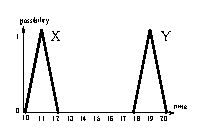
\includegraphics[scale=1.5]{graphs/ill-known-ti.eps}
   \caption{An ill-known time interval IKTI $J = \left[X, Y  \right]$ given by two ill-known values. }
   \label{fig:ill-known-ti}
 \end{figure}

\begin{definition}
An ill-known time interval \emph{(IKTI)} is defined by two ill-known values (see Figure \ref{fig:ill-known-ti}). Therefore, both starting and ending points are not precissely known. The following is the notation for an IKTI.

\begin{align}
\label{eq:ill-known-time-interval}
J = \left[X, Y \right] 
\end{align}

Where both $X$ and $Y$ are ill-known time values.
\end{definition}

The Allen's Relations between a crisp time interval $I = [a,b]$ ($a, b$ are crisp time points) and an IKTI given by $J = [X,Y]$ ($X, Y$ are ill-known values, see Definition \ref{def:ill-known-value}) can be defined by using aggregations of ill-known constraints. Table \ref{tab:allen-relations} shows the corresponding ill-known constraints for each Allen's Relation. These ill-known constraints are aggregated by using the equations \eqref{and-ill-known-pos} to \eqref{not-ill-known-nec}.



\begin{table}[h]
\centering
\begin{tabular}{|c|c|c|}
\hline
Allen Relation & Constraints & Aggregation \\
\hline
I before J & $C_1\stackrel{\triangle}{=} \left(<,X\right)$ & $C_1(I)$ \\
\hline
\multirow{4}{*}
{I equal J} & $C_1\stackrel{\triangle}{=} \left(\geq,X\right)$ & $C_1(I)\wedge$\\
 & $C_2\stackrel{\triangle}{=} \left(\neq,X\right)$ & $\neg C_2(I)\wedge$\\
 & $C_3\stackrel{\triangle}{=} \left(\leq,Y\right)$ &  $C_3(I)\wedge$ \\
 & $C_4\stackrel{\triangle}{=} \left(\neq,Y\right)$ & $\neg C_4(I)$\\
\hline
\multirow{2}{*}
{I meets J} & $C_1\stackrel{\triangle}{=} \left(\leq,X\right)$ & $C_1(I)\wedge$\\
 & $C_2\stackrel{\triangle}{=} \left(\neq,X\right)$ & $\neg C_2(I)$\\
\hline
\multirow{3}{*}
{I overlaps J} & $C_1\stackrel{\triangle}{=} \left(<,Y\right)$ & $C_1(I)\wedge$\\
 & $C_2\stackrel{\triangle}{=} \left(\leq,X\right)$ & $\neg C_2(I)\wedge$\\
 & $C_3\stackrel{\triangle}{=} \left(\geq,X\right)$ & $\neg C_3(I)$\\
\hline
\multirow{4}{*}
{I during J} & $C_1\stackrel{\triangle}{=} \left(>,X\right)$ & $\big(C_1(I)\wedge$\\
 & $C_2\stackrel{\triangle}{=} \left(\leq,Y\right)$ & $ C_2(I)\big)\vee$ \\
 & $C_3\stackrel{\triangle}{=} \left(\geq,X\right)$ & $\big(C_3(I)\wedge$ \\
 & $C_4\stackrel{\triangle}{=} \left(<,Y\right)$ & $C_4(I)\big)$\\
\hline
\multirow{2}{*}
{I starts J} & $C_1\stackrel{\triangle}{=} \left(\geq,X\right)$ & $C_1(I)\wedge$\\
 &  $C_2\stackrel{\triangle}{=} \left(\neq,X\right)$ & $\neg C_2(I)$\\
\hline
\multirow{2}{*}
{I finishes J} & $C_1\stackrel{\triangle}{=} \left(\leq,Y\right)$ & $C_1(I)\wedge$\\
 & $C_2\stackrel{\triangle}{=} \left(\neq,Y\right)$ & $\neg C_2(I)$\\
\hline
\end{tabular}
\caption{Allen's relations represented in the framework.}
\label{tab:allen-relations}
\end{table}

% \subsection{\label{subsec:ill-known-time-interval}Ill-known time intervals}
% The representation of an ill-known time interval is made by using two ill-known values. Therefore, both starting and ending points are not precissely known. Usually, a crisp interval $[a, b]$ is defined by using a constraint ($a \leq b$). In the case of ill-known intervals, an ill-known constraint is defined.

%%%
%%% Define ill-known time interval in an informal way.
%%%
%%%




% \subsection{Interval Evaluation by Ill-known Constraints}
% The problem of interval evaluation is more generally explained in \cite{Pons2011}: the need exists to know if all points in a crisp interval $I$ reside between the boundaries of an ill-known interval $\left[ X , Y \right]$. In \cite{Pons2011}, the notion of an \emph{ill-known constraint} is introduced:
% 
% \begin{definition}
% Given a universe $U$, an ill-known constraint $C$ on a set $A \subseteq U$ is specified by means of a binary relation $R \subseteq U^{2}$ and a fixed, ill-known value denoted by its possibilistic variable $V$ over $U$, i.e.:
% \begin{align}
% C \triangleq (R,V)
% \end{align}
% Set $A$ now satisfies the constraint if and only if:
% \begin{align}
% \forall a \in A : (a,V) \in R
% \end{align}
% \end{definition}
% 
% An example of an ill-known constraint is $C_{ex} \triangleq (<, X)$. Some set $A$ then satisfies $C_{ex}$ if $\forall a \in A : a < X$, given possibilistic variable $X$.
% 
% The satisfaction of a constraint $C \triangleq (R,V)$ by a set $A$ is basically still a Boolean matter, but due to the uncertainty about the ill-known value $V$, it can be uncertain whether $C$ is satisfied by $A$ or not \cite{Pons2011}. In fact, this satisfaction now behaves as a proposition. Based on the possibility distribution $\pi_{V}$ of $V$, the possibility and necessity that $A$ satisfies $C$ can be found. This proposition can thus be seen as a possibilistic variable on $\mathbb{B}$. The required possibility and necessity are:
% 
% \vspace{-10pt}
% 
% \begin{align}
% \Pos(A\text{ satisfies }C) & = \min_{a \in A}\left(\sup_{(a,w) \in R}\pi_{V}(w)\right) \label{ill-known-pos}\\
% \Nec(A\text{ satisfies }C) & = \min_{a \in A}\left(\inf_{(a,w) \notin R} 1-\pi_{V}(w)\right) \label{ill-known-nec}
% \end{align}
% 
% Now, e.g., to check if crisp interval $I = \left[j, k\right]$ is included in $\left[X, Y\right]$, 2 ill-known constraints are constructed:
% 
% \vspace{-10pt}
% 
% \begin{eqnarray}
% C_1 & \triangleq\left(\geq,X\right)\\
% C_2 & \triangleq\left(\leq,Y\right)
% \end{eqnarray}
% 
% To calculate the possibility and necessity concerning a conjunction of constraints, the $\min$ operator can be used. The possibility and necessity of $I$ being included in $\left[X, Y\right]$ are now: 
% 
% \vspace{-10pt}
% 
% \begin{align}
% \label{eq:interval-pos}
% \Pos(I\text{ satisfies }C_1\ and\ C_2) & = \min_{a \in I}\left(\sup_{a \geq w}\pi_{X}(w),\sup_{a \leq v}\pi_{Y}(v)\right)\\
% \label{eq:interval-nec}
% \Nec(I\text{ satisfies }C_1\ and\ C_2) & = \min_{a \in I}\left(\inf_{a < w} 1-\pi_{X}(w),\inf_{a > v} 1-\pi_{Y}(v)\right).
% \end{align}

